% Activate the following line by filling in the right side. If for example the name of the root file is Main.tex, write
% "...root = Main.tex" if the chapter file is in the same directory, and "...root = ../Main.tex" if the chapter is in a subdirectory.
 
%!TEX root =  testMain.tex

\chapter[Simple Spatial Simulations]{A Simple Robbery - Spatial Simulations and their Bayesian Networks}

 The problem is that in the previous chapter, we have established that we have a method to convert a simple forward-chaining simulation into a collection of data, which then in turn can be used to create a Bayesian Network, that represents the situation in the simulation.
 
 However, this was totally 100\% determined by deterministic forward chaining rules. The real world does not run on deterministic forward chaining rules (as far as we know). At least, we are spatially situated, which means that there are probabilities that will arise out of interactions between agents and their environment. These probabilities are not `set' in the same ways as the probabilities are set in the previous chapter, they arise organically from interactions: an agent has to be located at a door to break in, an agent can be seen by a camera only in some locations of the simulation. We do not know these probabilities a-priori.
 
 Research questions for this chapter:
 
 \begin{itemize}
 \item Can we create an automatic BN from a simulation of similar accuracy and rmse as in the previous chapter, but now spatially explicit, with agents, and with evidence?
 \item What is the effect of loss of precision on this network?
 \item What is the effect of truly private knowledge on the network?
 \end{itemize}
 


\section{Experiment 1: Generating BNs and lowering precision}

For the first experiment, a very simple crime case will be modelled in a multi-agent simulation. This is the data-generating environment, the gathered data will be used by the K2 algorithm to automatically generate a Bayesian Network. This network will be assessed based on the criteria set out in chapter 3.  

\subsection{Introduction}

The scenario that the agents play out goes as follows. There are two agents. They are neighbors. One day, the agent who lives in the house on the right ($R$), walks past the house of the other agent ($L$). $R$ looks inside, if it can. Sometimes it cannot look inside, because $L$ has drawn the curtains. However, if $R$ can look inside, it might see a goodie in the house. It also might not see a goodie, if $L$ has lost the goodie - in that case, the goodie has been lost. However, if the goodie is there, $R$ will know that the goodie is there. Then, because $R$ is a rational agent, it will try to calculate the worth of the object, and if it might want to steal it. It can decide to target the object. If $R$ knows and targets the object, $R$ has a motive. Then, $R$ attempts to break into the house by breaking the lock on the door, grabbing the goodie, and running away to its own house.  Meanwhile, $L$ is returning home. If $R$ thinks that $L$ might have seen it stealing, $R$ will flee home, with or without the goodie. $L$ has also hung up security cameras on the outside corner of its house, that might serve as evidence against $R$.

With regards to the end, there can be three outcomes: either the goodie is lost, the goodie is not lost but was stolen successfully, or the goodie is not lost and wasn't stolen successfully. %({\color{red}does this mean that there was always a stealing attempt? check in jup}). 
The environment of the agents is very simple, just two `houses' (rectangles, really). The environment and the agents (with their vision parameter) are shown in Figure~\ref{env}.

\begin{figure}[htbp]
\begin{subfigure}{.5\textwidth}
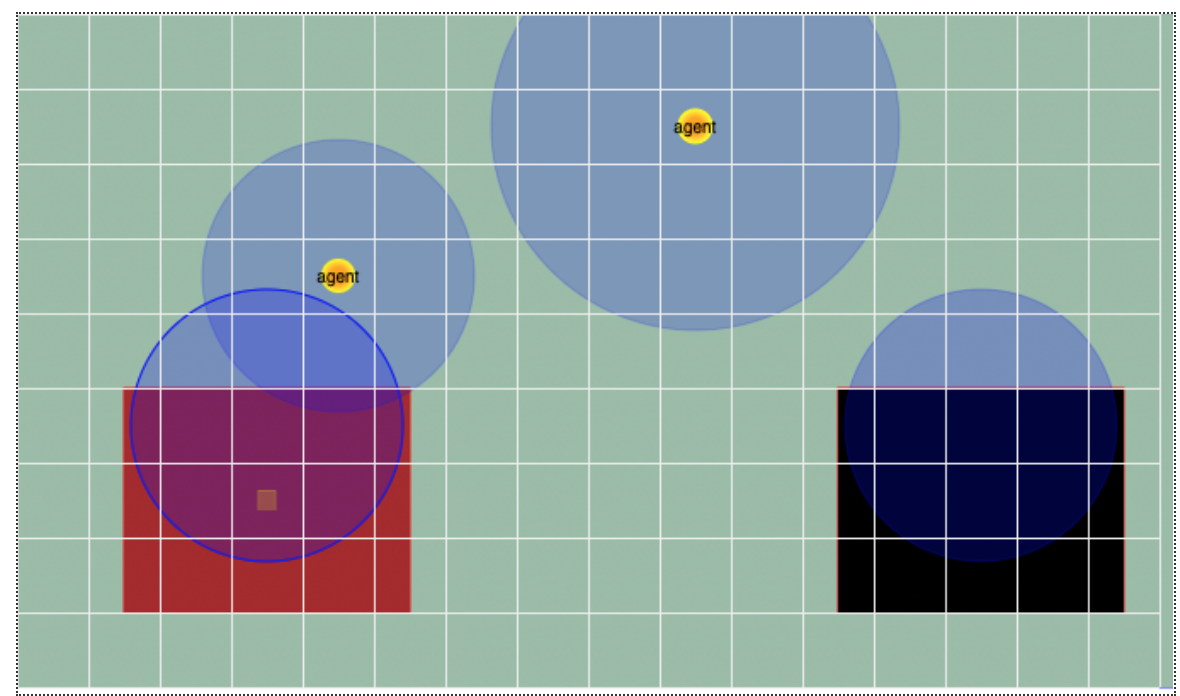
\includegraphics[width=\linewidth]{images/sim1.png}
\caption{The simulation with the 2 agents.}
\end{subfigure}
\begin{subfigure}{.5\textwidth}
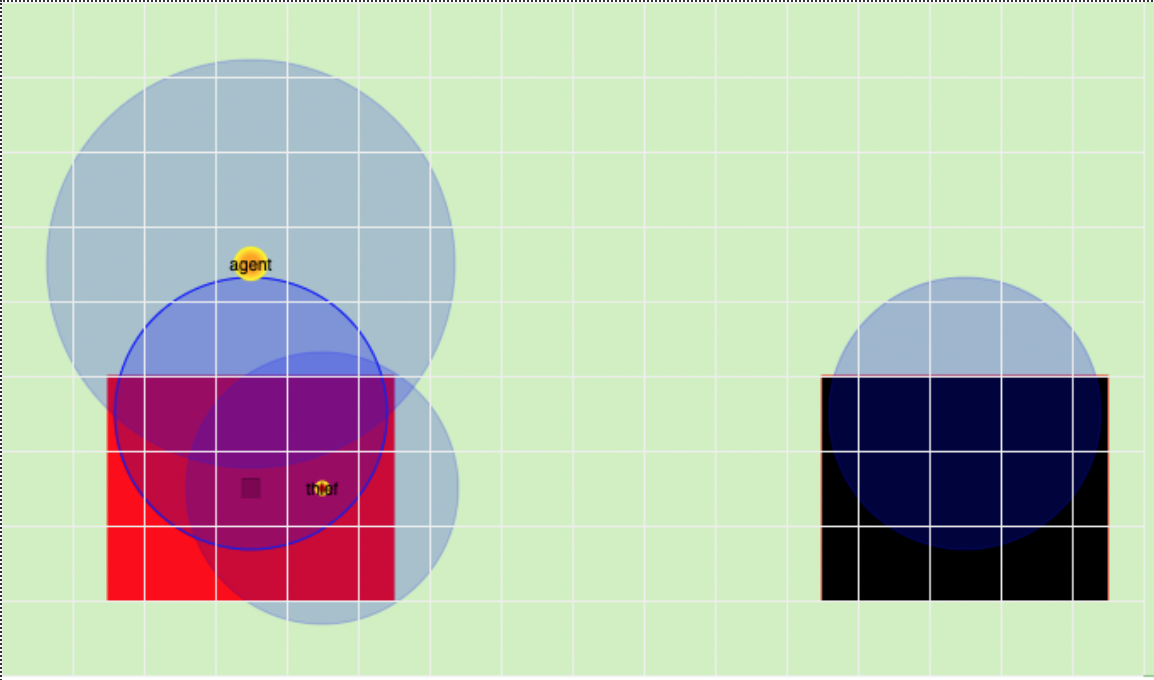
\includegraphics[width=\linewidth]{images/stealing.png}
\caption{The agent attempts to steal something but flees when it thinks that it is noticed.}
\end{subfigure}
\caption{Agents behaving badly in simulation.}
\label{env}
\end{figure}

\subsection{Methods}

We created a simulation of the situation described in the introduction, using the MESA multi-agent framework in Python. There are two agents, who are walking around in a discrete grid. Every simulation was simulated for 30 epochs, because all the possible scenarios could be described within 30 epochs. We performed 2000 iterations. 

The behaviour of the agents is described in Figure~\ref{behaviour}. 

\begin{figure}[htbp]
\begin{center}
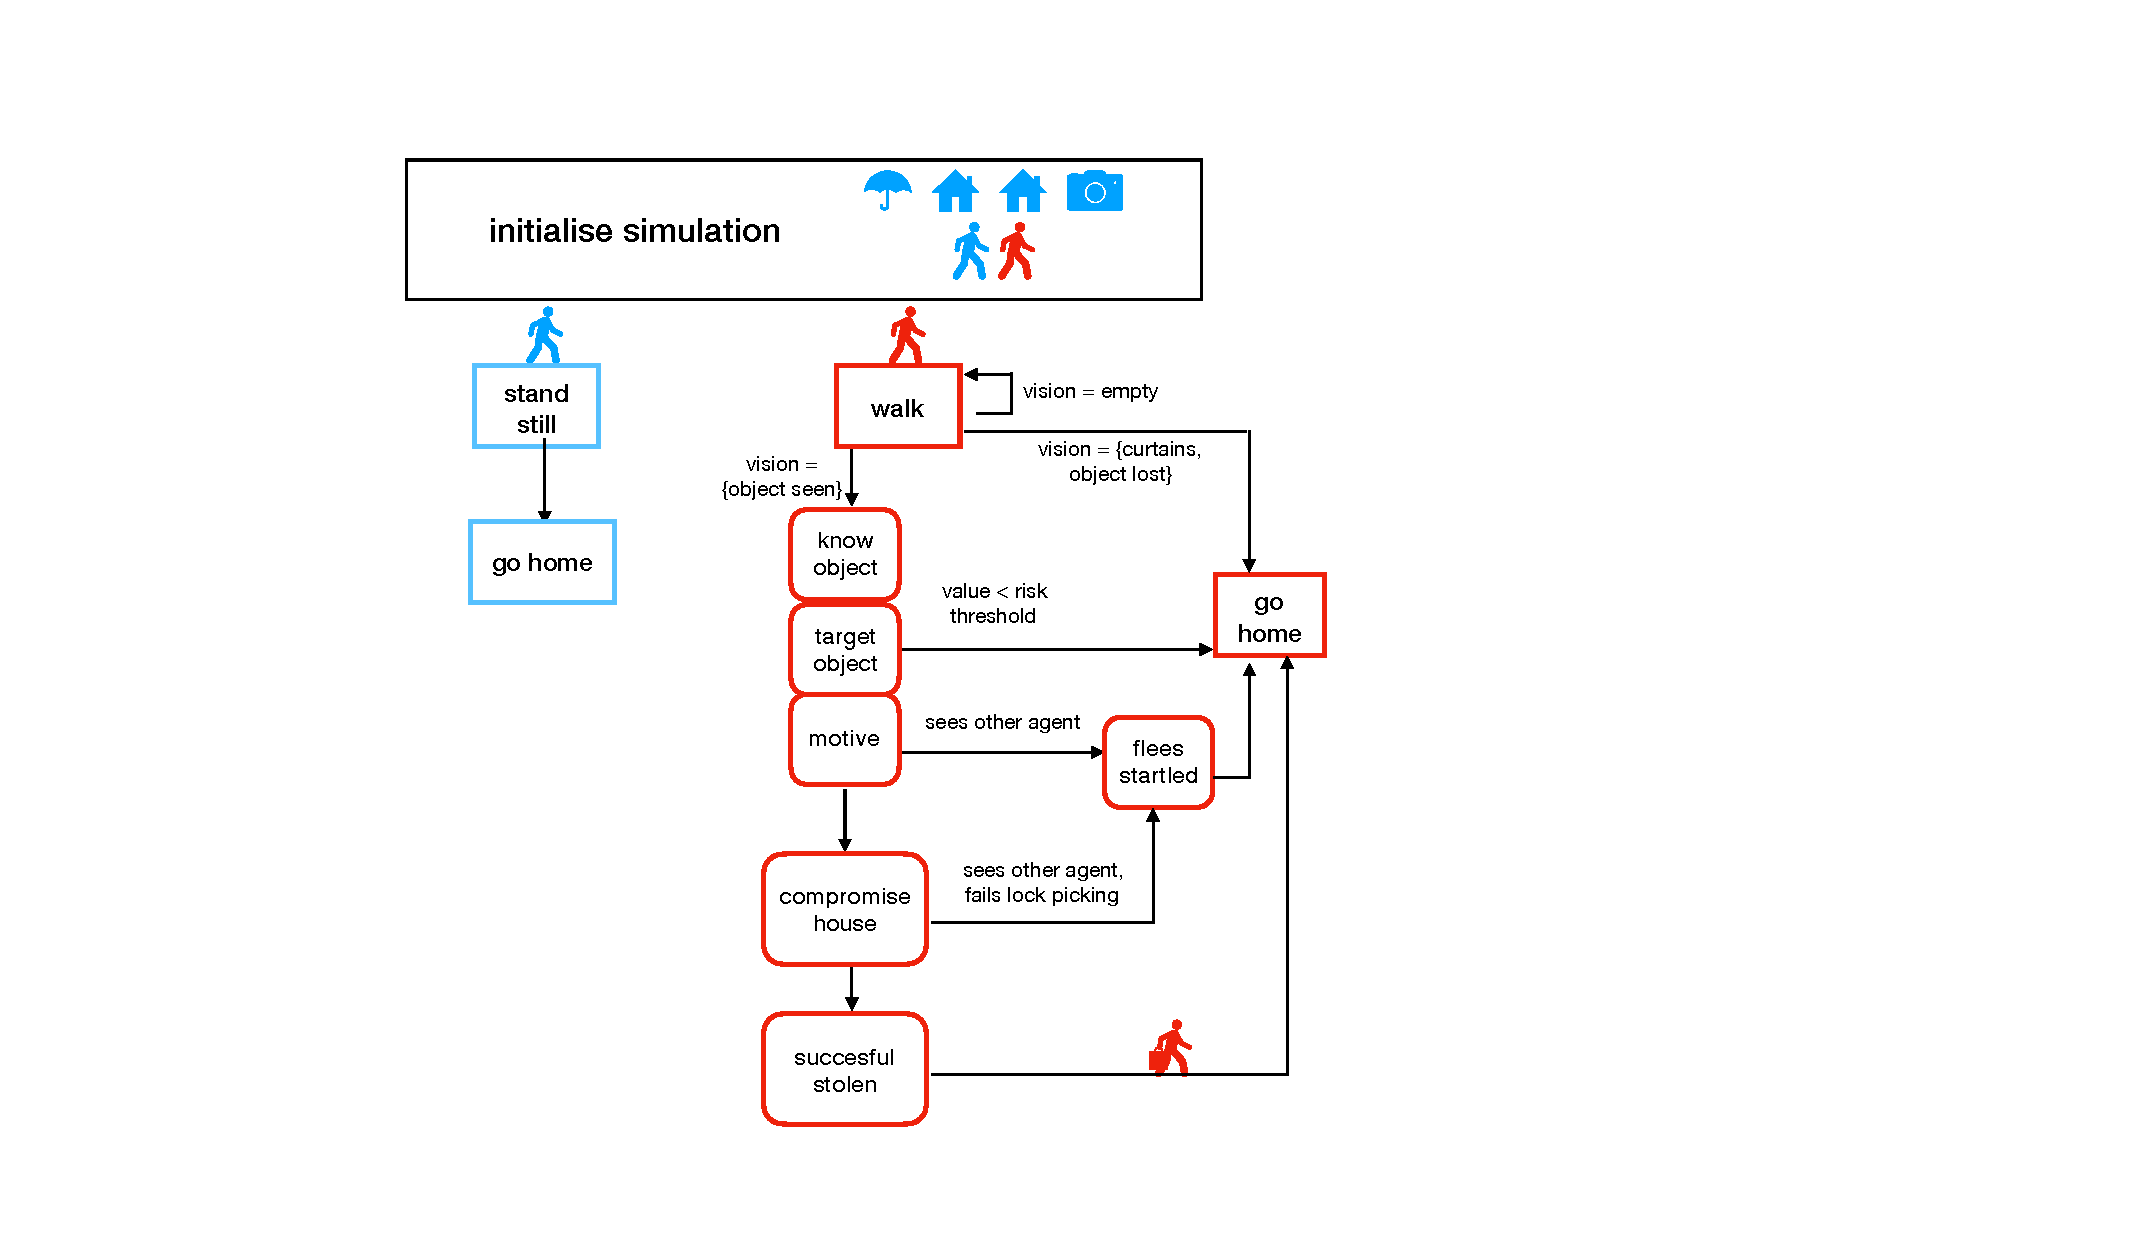
\includegraphics[width=\linewidth]{images/spatialsimpleAgent.pdf}
\end{center}
\caption{The behaviour of the agents. The nodes with rounded edges correspond to the nodes in the Bayesian Network.}
\label{behaviour}
\end{figure}

The actions of the agents correspond to reporters. The operationalisation of the reporters (random variables) are described below:

\begin{adjustbox}{center}
\footnotesize
%\centering
\begin{tabular}{|l|l|}
 \hline
 RV &Operationalization\\
 \hline
lost\_object   & A random number generator (0, 1) generates a number. If the number $\leq 0.2$, the object is lost.\\
curtains & A random number generator (0, 1) generates a number. If the number $\leq 0.8$, the house has no curtains.  \\
raining & A random number generator (0, 1) generates a number. If the number $\leq 0.5$, it is raining.   \\
know\_object & if we see an object in our vision that is not our own, and we are not already targeting some`
thing else  \\
target\_object & if we know the object exists, and we consider the value of the object higher than our risk threshold.  \\
motive & if we have a target \\
compromise\_house & if we are adjacent to the target's house's door, and we have a breaking and entering skill of greater than 5. \\
flees\_startled & if we see another agent and we haven't been observed yet  \\
successful\_stolen & if we're not in someone's house anymore and we have the object in our possession \\ 
E\_s\_spotted\_by\_house&  {\color{red} todo fill in}. \\ 
E\_disturbed\_house&   \\ 
E\_object\_is\_gone&   \\ 
E\_broken\_lock&   \\ 
E\_s\_spotted\_with\_goodie&   \\ 
E\_private&   \\ 
\hline
\end{tabular}
\end{adjustbox}


\subsection{Results}

The generated Bayesian Network is shown in Figure~\ref{laptop}.

\begin{figure}[htbp]
\begin{center}
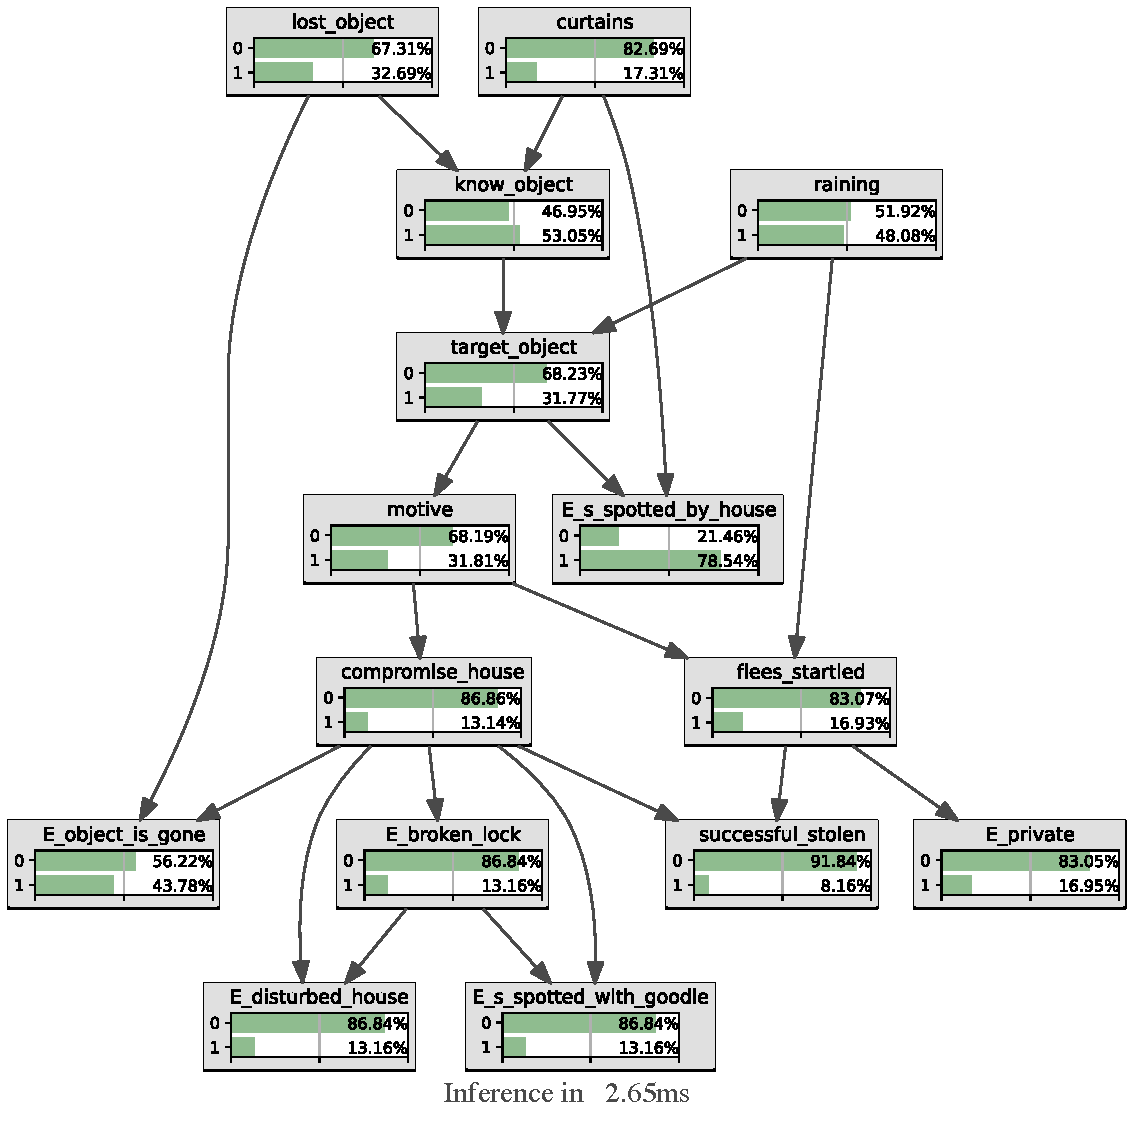
\includegraphics[width=\linewidth]{../experiments/StolenLaptop/bnImage/BNIMAGEStolenLaptop.pdf}
\end{center}
\caption{network structure}
\label{laptop}
\end{figure}


\subsubsection{Evaluation with regards to structural, performance and human-factor criteria}
In this section, the evaluation criteria as set out before are applied to the networks.

\subsubsection{Structural Criteria}
\begin{enumerate}
\item \textbf{Hypotheses are ordered temporally.}

The main scenario hypothesis nodes are ordered temporally.

\item \textbf{Evidence connects to hypotheses.}

All evidence is connected to at least one hypothesis. However, the structure of how the evidence nodes are added is confusing and overwhelming. One piece of evidence - the most crucial one, which is that the evidence is gone, has 5 parents!

\item \textbf{Relevance: All relevant events are in the BN, all irrelevant events are outside of the BN.}

We know that truly irrelevant nodes are kept out of the main Bayesian Network - we can see that the node for `raining' is not connected to any other node. This is because the rain does not affect anything in this simulation - this is reflected in the Bayesian Network.

\item \textbf{Independent events are not connected to each other.}

Evidence is connected to each other. This is because we need to consider dependent evidence as dependent in the network (see \citep{Fenton2012} for explanation of dependent evidence).

\end{enumerate}


%%%%%%% Criteria %%%%%%%%
\subsubsection{Performance Criteria}
We consider the accuracy and root mean square per network, then also look at the correspondence, sensitivity values and the progression given a certain evidence set.
\begin{enumerate}
\item \textbf{Accuracy and Root Mean Square error}

The accuracy of the network is 87.9\% and Root Mean Square error is 0.14. This is comparable to the networks in the previous chapter.

\item \textbf{Correspondence.}

Once again, compared the probabilities in the network with the frequencies of the events in the simulation (maybe run again, larger training set but don't actually train on it). We see the same pattern (Table~\ref{test}) as before, it is accurate within ±0.005. 

\begin{table}
\centering
\begin{tabular}{|c|c|c|}
 \hline
 Conclusion & Frequency P(event) & BN P(event)\\
 \hline
lost\_object   & 0.1985 & 0.1987\\
curtains & 0.1695 &  0.1697\\
raining & 0.5085 &  0.5085\\
know\_object & 0.6515 &  0.6510\\
target\_object & 0.3135 & 0.3134\\
motive & 0.3135 & 0.3133\\
compromise\_house & 0.0925 & 0.0925 \\
flees\_startled & 0.1655 &  0.1654\\
successful\_stolen & 0.05 & 0.0438\\ 
E\_s\_spotted\_by\_house&  0.901 & 0.9004 \\ 
E\_disturbed\_house& 0.071 &  0.0709\\ 
E\_object\_is\_gone&  0.281 &  0.2793\\ 
E\_broken\_lock&  0.0925 &  0.0924\\ 
E\_s\_spotted\_with\_goodie& 0.083  & 0.0813 \\ 
E\_private&  0.1655 & 0.1653\\ 
\hline
\label{test}
\end{tabular}
\caption{Correspondences}
\end{table}


\item \textbf{Sensitivity analysis values}

\item \textbf{Effect of evidence on the posterior.}

The effect of turning on evidence on the posterior of the initial network is shown in Figure~\ref{baseposterior}.

The scenario that this posterior progression corresponds to is as follows: the duped agent comes home, and finds that their object is gone. Then, it takes a closer look at the door, and sees that the lock is broken. It looks at the disturbed house, and then at the cameras. The camera shows that the other agent was spotted near the house, and later on emerged with the object. Then, we need to look inside the head of the stealing agent, who fled before they saw the duped agent come home - hence, E\_private is 0.

We see the effect of evidence strength in this progression: once we know that the lock is broken, seeing that the house is disturbed does not add anything to our estimation of the posterior of being robbed, and spotting the suspect near the house also does not change the posterior. Only when we see the suspect with the robbed object, the posterior starts to increase again. This corresponds to intuition.

\begin{figure}[htbp]
 \centering
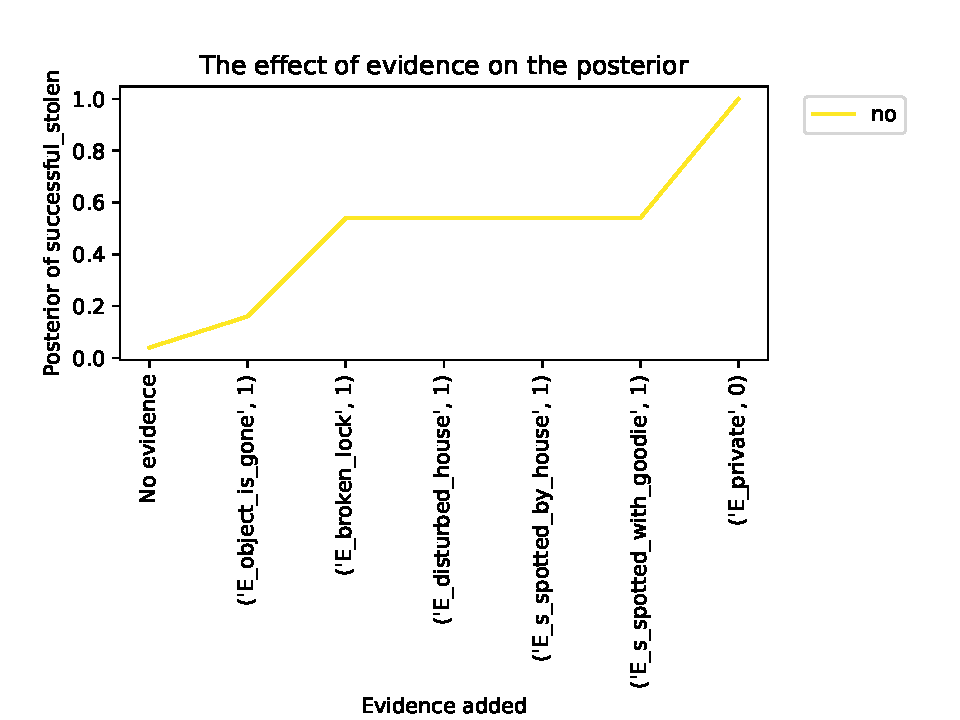
\includegraphics[width=0.6\linewidth]{../experiments/StolenLaptop/plots/posterior_base_networkStolenLaptop.pdf}
\caption{ Progression of evidence resulting in changing the posterior}
\label{baseposterior}
\end{figure}%


\end{enumerate}

\subsubsection{Human Criteria}
\begin{enumerate}
	\item \textbf{How robust is the network against a loss of precision?}

	We again create networks with lower precision, and use the $\epsilon$ method to create networks that do not saturate with 1 or 0, like in the previous chapter. Then we calculate accuracy and root mean square errors on lower-precision networks (Figure~\ref{dist}). We again see that while the RMSE increases when we lose precision, it does not increase by much - from 0.14 to 0.20. Rounding to $\epsilon$ and $1-\epsilon$ instead of 0 or 1 results in robust networks that keep the same accuracy even under loss of precision. So this method works even for more complex networks that include evidence. 
	
	The posterior progression is also relatively the same as the original network (Figure~\ref{post}), only with some variation: the nuances in evidence strength are flattened-out: we see that for networks with less precision (like those rounded to 0.5 and 0.33), there are only 4 points where the value of the posterior changes, while for more precise networks, like the BN rounded to 0.05, the posterior changes value in 6 places. 
	
	\begin{figure}[htbp]
\begin{center}
\begin{subfigure}{.5\textwidth}
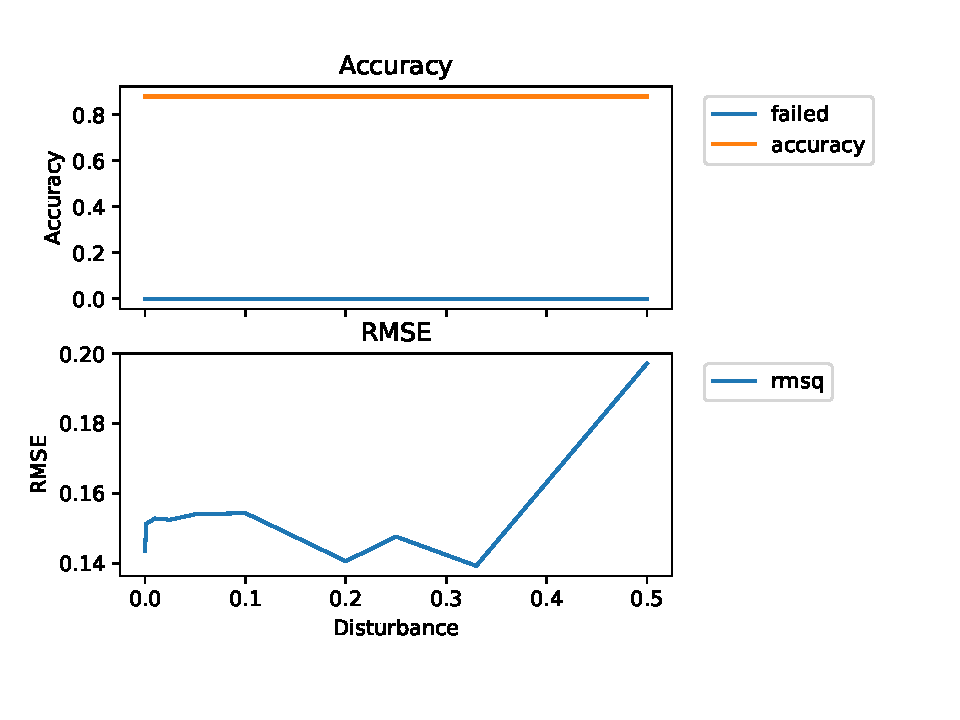
\includegraphics[width=0.9\linewidth]{../experiments/StolenLaptop/plots/performance_StolenLaptop.pdf}
\caption{Network Under Disturbance.}
\label{dist}
\end{subfigure}%
\begin{subfigure}{.5\textwidth}
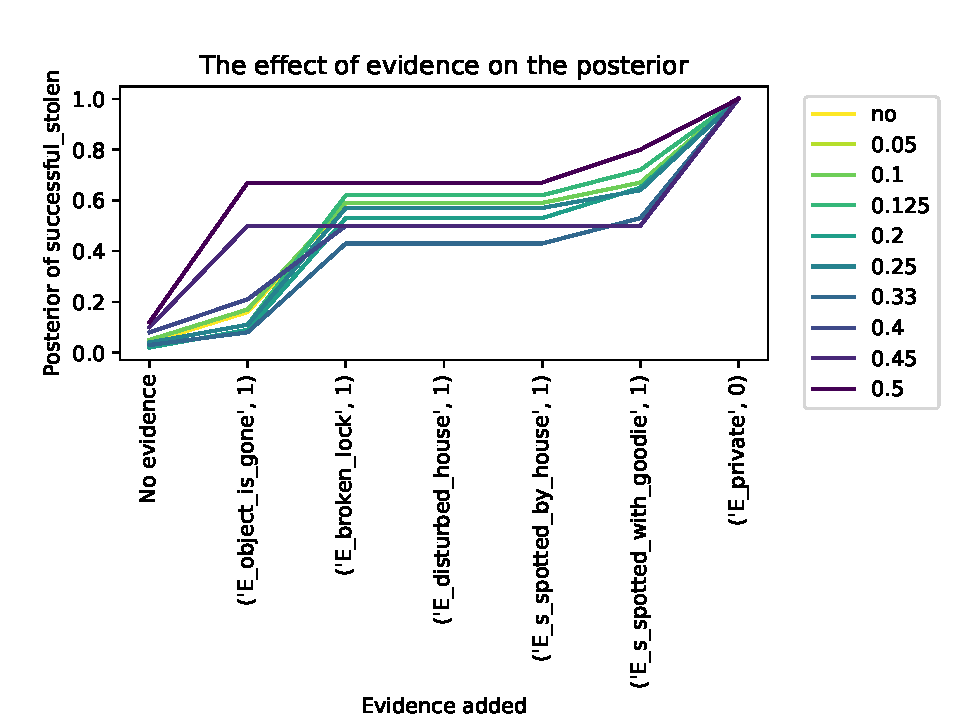
\includegraphics[width=0.9\linewidth]{../experiments/StolenLaptop/plots/posterior_StolenLaptop.pdf}
\caption{ Progression of evidence resulting in changing the posterior}
\label{post}
\end{subfigure}
\end{center}
\caption{Loss of precision in networks.}
\end{figure}

	\item \textbf{Could a human modeller find these probabilities?}
	Due to the high accuracy and similar posterior progression of the lower-precision networks, it is not essential that a modeller finds precise probabilities.
	
	\item \textbf{ Can a human modeller determine the correct independence relations?}
	This is more difficult - the way that evidence is connected to the hypotheses is complex and confusing. Additionally, there are sibling-nodes (nodes with the same parents), and how these nodes relate to each other temporally cannot be understood from the BN alone (does compromise house come before or after flees startled?). 
\end{enumerate}

\subsection{Discussion}
We have shown that we can model spatial simulations with agents and evidence to a reasonable accuracy (88\%) in a Bayesian Network. The network generally fulfils the criteria we set out for it: The generated network is ordered temporally, complete, includes evidence, has a high accuracy, and performs well under lower precision.

 Only the connections of the evidence to the network is confusing and complex. The cpts in the network can become less precise without losing accuracy, which is promising for elicitation. However, lower precision in the network reduces expression and nuance of evidence strength.
 
  \begin{table}[htp]
\begin{center}
\begin{tabular}{|c|c|c|c|}
 \hline
 Network & Accuracy & Root Mean Square & Inconsistency error\\
 \hline
 Stolen Laptop   & 0.499 &  0.50 & 0   \\
\hline
\end{tabular}
\caption{Accuracy and Root Mean Square Error for the networks calculated on the impossible states.}
\end{center}
\label{tabB}
\end{table}


\section{Experiment 2: Investigating Private Knowledge}

This experiment tests the effect of private knowledge on the resulting network and its accuracy and ability to get to a posterior.

\subsection{Introduction}
We can think about the process of a criminal investigation and a trial as a systemic way of gathering, sharing and finally agreeing on knowledge. Initially, only the criminal will know the entire story, victims know parts of it, and the police and judges know even less. An ideal trial results in common knowledge of the entire situation.

Of course, it is not in the interest of everyone to freely share their private knowledge all the time. Police might not want to talk about the limitations of their evidence (or their ways of procuring it), witnesses and victims might not want to talk due to incrimination, shame, or relationships to the people involved. Suspects might not want to freely share their murder plans (obviously). There is an abundance of private knowledge.

 The Bayesian Network generated up till now, have not taken this into consideration. We have the full set of nodes - even nodes that a realistic investigation cannot be sure about, like the internal considerations of the criminal agent (who will flee when it sees the other agent). If we were real investigators, we cannot actually know this behaviour and model it in our network before the agent admits to the behaviour in court.
 
 This would imply that we can only create Bayesian Networks after the fact: only when the court case is over, and all the facts and their probabilities have been established, can we start building them. Otherwise, we risk missing out on essential psychological or internal information. This would not be ideal. This leads us to ask the question: do our networks still work if we lose information about the internal intentions of agents?

\subsection{Method}
We identify the nodes `flees\_startled' and `E\_private' as events that can only be established after the fact. The reporters for these nodes are disabled and not included in the data that is passed to the K2 algorithm. This means that the network-building algorithm does not even know of the existence of these nodes, and will generate an entirely new network based on all the other nodes, except these two. The behaviour of the agents and the simulation remains the same.

\subsection{Results}
The resulting Bayesian Network is presented in Figure~\ref{privatelaptopN}. The complexity of this network is lower than the initial network because the two nodes are missing. However, even though there is information missing from the network, the accuracy and RMSE of the network, even under lower precision, are comparable to the initial network: 87.5\% and 0.13 (Figure~\ref{privatelaptopA}).

The important difference between this network and the full network is the response of the posterior (Figure~\ref{privatelaptoppost}). In the full network, once all the evidence was entered, we found a posterior probability for `stolen successfully' to be 1, for all precisions. However, in this situation, since essential evidence is missing, the posterior probability for `stolen successfully' is reduced to 80\%, and cannot be increased any further. 

\begin{figure}[htbp]
\begin{center}
\begin{subfigure}{.50\textwidth}
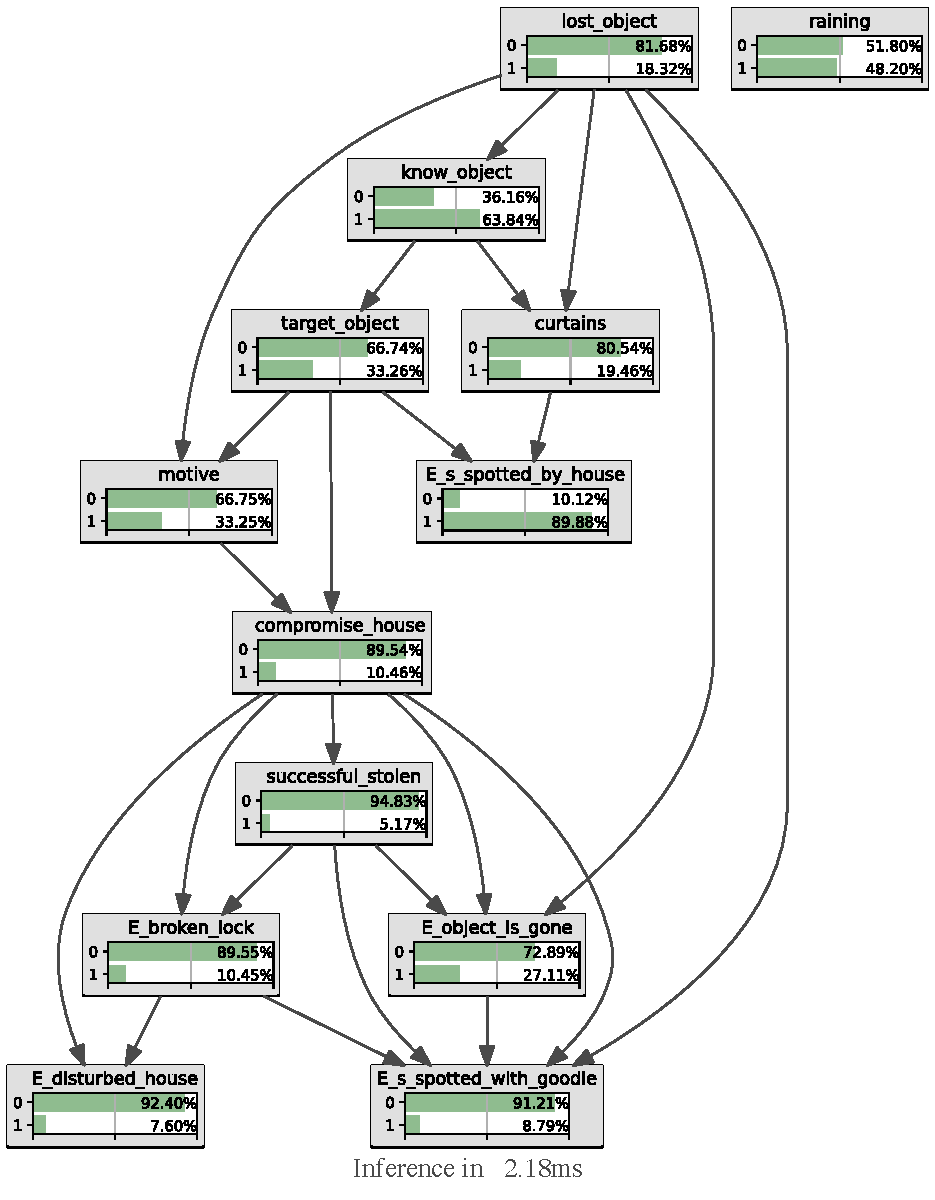
\includegraphics[width=\linewidth]{../experiments/StolenLaptopPrivate/bnImage/BNIMAGEStolenLaptopPrivate.pdf}
\caption{network structure for missing private information}
\label{privatelaptopN}
\end{subfigure}
\end{center}

\begin{subfigure}{.45\textwidth}
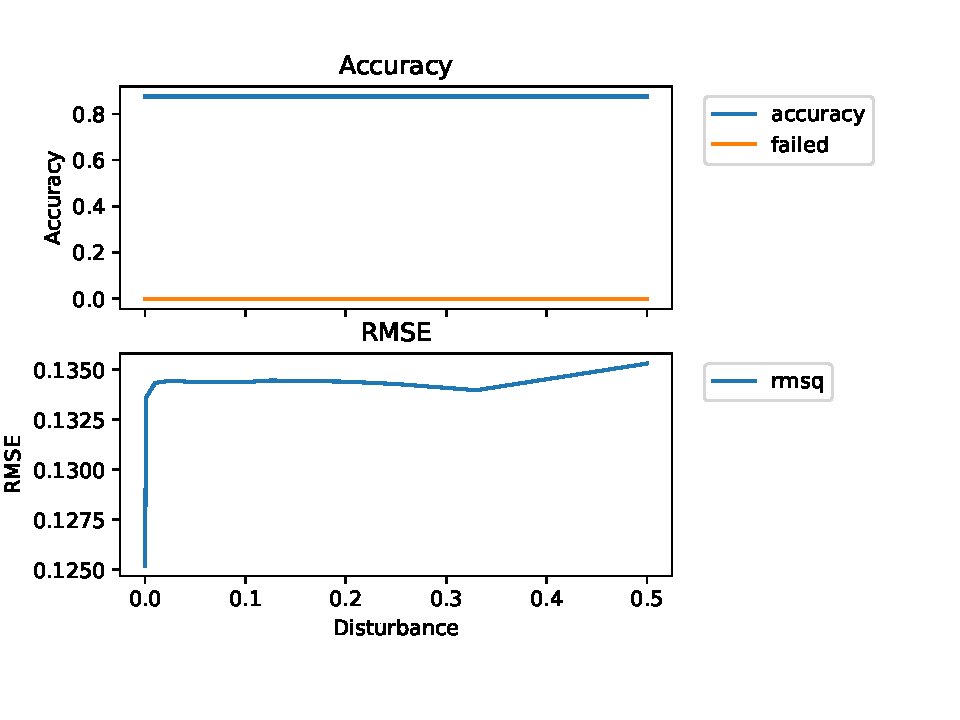
\includegraphics[width=\linewidth]{../experiments/StolenLaptopPrivate/plots/performance_StolenLaptopPrivate.pdf}
\caption{Accuracy (100\% to 0\%) and Root Mean Square error (1 - 0) for missing private information}
\label{privatelaptopA}
\end{subfigure}%
\begin{subfigure}{.45\textwidth}
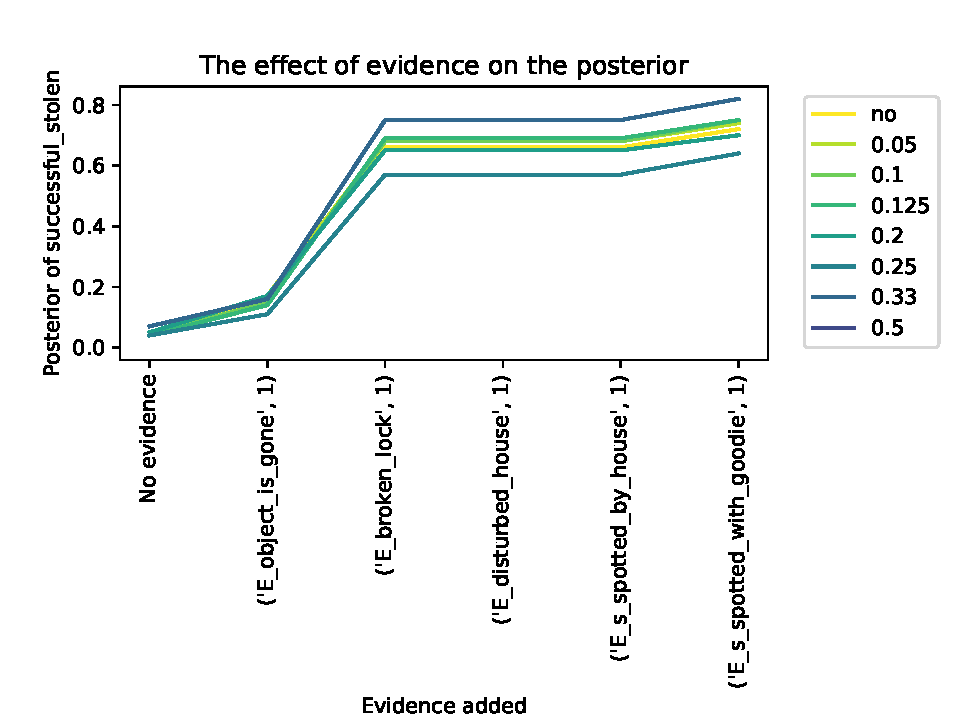
\includegraphics[width=\linewidth]{../experiments/StolenLaptopPrivate/plots/posterior_StolenLaptopPrivate.pdf}
\caption{posterior private information}
\label{privatelaptoppost}
\end{subfigure}

\caption{The network, the accuracy and root mean square for rounding the cpts to intervals, and the effect of evidence on the posterior for stolen laptop simulation.}
\label{private}

\end{figure}


\subsection{Discussion}
Losing essential evidence from the network does not reduce its accuracy or increase RMSE, even under lower precision. Even though the accuracy of the network remains high when we miss private knowledge, the lack of private knowledge has important implications. We see that the probability of the posterior when all evidence is added is 0.8. It dips below the 0.95\% posterior probability that is seen by \citet{Fenton2019} as the required posterior probability for determining guilt. The initial network did not have this problem. This implies that there is a fundamental uncertainty in the BN (which is true, because we are missing nodes), and we cannot be fully sure that the object was stolen. We are only fully sure when the posterior of `stolen\_successfully' goes to 1.

We are also too charitable with our interpretation of what private knowledge is. We only took `flees startled' and the evidence for it, but in real life there are many things that are private knowledge. Nodes like `target\_object' can only be truly known when we look into the suspect's head, and while we might consider that a suspect must always have a motive, the operationalization of a `motive' node in a real BN would be very difficult, because it is not clear how one would measure that a suspect has a motive.



\section{Discussion}

In this chapter, we have shown that we can build and experiment with Bayesian Networks that are generated from spatial multi-agent simulations with evidence. Even at lower precision, the networks perform well, although how evidence should be connected to the hypotheses remains an open question. 

In these networks, we see that the evidence updates the posterior in the right direction - more evidence for stealing leads towards a higher value of `successful-stolen'. We also see the effects of different evidence strengths - knowing that the lock is broken is more important than seeing that the house is disturbed.

The effect of private knowledge on the generation and accuracy of the network is also more clear: it does not affect accuracy, because we can round. However, we see that we cannot get the posterior for `stealing' as high as with the private evidence.





\subsection{Possible Legal Interpretations.}
% how will a judge interpret this
We have shown that this type of Bayesian Network does not have to be precise. This leaves room for disagreements about probabilities. We can imagine a trial where two experts have to make a subjective probability estimation. Due to the finding that lower precision does not impede accuracy very much, we now have more room for disagreement. If expert one thinks that some event is 20\% likely, and expert two thinks that the event is 30\% likely, they might still be able to agree on 25\%, and be happy with the resulting cpt for the event. Given this network, this would not reduce the accuracy of the network in predicting the outcome (although it might reduce the RMSE).  

However, we run into trouble when we want to be exact about a threshold for guilt. As we have seen in comparing experiment 1 to experiment 2, we see that we cannot increase the posterior for `stealing' in experiment 2 higher than 0.8, due to the lack of essential but private knowledge. In experiment 1, we can get this posterior to 1 with a lack of precision. We might have grounds to accept guilt in experiment 1, given the set of evidence that we showed, but do we have ground in experiment 2? 

If we take for guilt a probability of 0.99, we do not, but in experiment 2 we can never reach a probability of guilt that is that high, because we miss essential information. It might be the case that if we build a network in which the final output probability can never be higher than 0.8, it could be a sign that we are missing essential information (like the lack of private knowledge), and our BN is not complete. This idea warrants further investigation.

The final and essential problem here is also something discussed in the previous chapter: the operationalisation and reference class of the events. In our simulation, we are taking this for granted, because our reporters work. We have the operationalisation, we know the reference class, and due to this we can automatically generate Bayesian Networks. However, in the real world we would find it difficult to properly operationalise many of these variables. How do we know if an agent is spotted `by a house'? Do we mean `we can see the agent on camera'?, but what if the camera has a large range and can see the other side of the street? How do we define `nearness'? How do we know that our methods for determining the truth or falsity of our events are valid? How do we decide which events we are selecting in the first place? These are all open questions that are not answered by this project.

%Forensic scientists will probably be annoyed by the lack of precision, but in these cases we do have a good operationalisation of what exactly is going on. Because we have this operationalisation, we can be sure that our data collection is correct. In the sci-fi world where police builds Bayesian Networks, I can imagine a situation where someone goes over all the files of all the crimes everyday, and collects statistics on occurances. However, the granularity of these crime files and the operationalisation are essential. Here, we can take them for granted. In real life, we cannot and that's a huge problem. 




%We run into problems when we use words like `near' in our node names. We're lucky that we know what we mean (because our reporter forces us to make this explicit). We do not just ground the probabilities in our network, but we actually also ground our random variables - we have a measure of exactly what events we are interested in, and which we aren't.

%We are in trouble with private knowledge, dropping this column from our table (which means that we don't know it) when we make our BN, we're drastically reducing our uh. Accuracy, and increasing our RMS. This implies that we do seem to need a full picture of everything that's happening, otherwise our BN will be kind of terrible, and be less accurate :(.

%Hence, for a simulation to work we 1) need to know exactly what it is that we're measuring since evidence strength depends on it \footnote{explain this more}, and 2) private information is necessary to create the BN because it influences fleeing behaviour. If we don't have this information our BN will be less effective.






